Dieser Abschnitt befasst sich mit dem aktuellen Stand der Technik. Dies umfasst
sowohl die gegenw{\"a}rtig eingesetzte Hardware, als auch bereits
entwickelte Protokolle zur Interplanetaren Kommunikation.


\textbf{Mars Rover Curiosity}

Der Mars Rover Curiosity (Abb. \ref{fig:Curiosity})verf{\"u}gt {\"u}ber einen
RAD750 Prozessor von BAE-Systems.
Dieser hat eine Taktfrequenz von bis zu 200 MHz und kann 266 MIPS oder mehr
verarbeiten. Desweiteren verf{\"u}gt Curiosity {\"u}ber einen Arbeitsspeicher von 256 MB
und einen Flash-Speicher von 2 GB. Zus{\"a}tzlich hat Curiosity einen EPROM von 256
KB. Alle Bauteile sind dabei besonders Strahlungsresistent und unempfindlich
gegen{\"u}ber gro{\ss}en Temperaturschwankungen. Das genutzte Betriebssystem ist
VxWorks. Zur Kommunikation nutzt der Rover
einerseits das X-Band (7 - 8 GHz), welches zur {\"U}bertragung von Statusdaten
und zum Empfang von Steuerdaten genutzt wird. Desweiteren verf{\"u}gt der Rover
{\"u}ber ein Kommunikationssystem im UHF-Band (0,4 GHz) welches f{\"u}
wissenschaftliche Daten mit hohem Datenvolumen genutzt wird (bis zu 250 Mbit
pro Tag, somit ca. 30 MB/Tag). Die Ausstattung an wissenschaftlichen
Instrumenten umfasst zehn Ger{\"a}te. Darunter z.B. zwei Mastkameras welche je
eine Aufl{\"o}sung von 1200 x 1200 Pixeln haben (1,44 Megapixel). Diese Kameras
sind ebenfalls in der Lage 720p-Videos mit einer Framerate von 10 Bildern pro
Sekunde aufzunehmen. Hinzu kommen Spektrografen, weitere Kameras, Sensoren etc.,
welche weitere Analysedaten beisteuern.

\begin{figure}[H]
\centering
\includegraphics[scale=.09]{Curiosity.png}
\caption{Mars Rover Curiosity}
\label{fig:Curiosity}
\end{figure}

\textbf{Deep Space Network}

Das Deep Space Network bezeichnet ein Netz von Parabolantennen, welche zur
Kommunikation mit Raumsonden, Satelliten sowie radio-
und radarastronomischen Zwecken dienen. F{\"u}r die NASA werden derzeit die
folgenden drei gro{\ss}en Stationen betrieben:

\begin{compactenum}[a)]
\item \textit{Goldstone Deep Space Communication Complex, Kalifornien, USA
(Abb.} \ref{fig:Goldstone}\textit{)}
\item \textit{Madrid Deep Space Communication Complex, Madrid, Spanien}
\item \textit{Canberra Deep Space Communication Complex, Canberra, Australien}
\end{compactenum}

Das Deep Space Network wird auch f{\"u}r die Kommunikation zwischen dem Mars
Rover Curiosity und der Erde genutzt. Die Anlagen liegen an exponierter Position
(zumei{\ss}t h{\"u}geliges schalenf{\"o}rmiges Gel{\"a}nde). Dies soll den
Einfluss von St{\"o}rungen z.B. durch Radiofrequenzen reduzieren. Die Stationen
befinden sich je in einem Abstand von einem drittel Erd{\"a}quator um eine
fortw{\"a}hrende Kommunikation mit Raumfahrzeugen trotz Erdrotation zu
erm{\"o}glichen.

\begin{figure}[H]
\centering
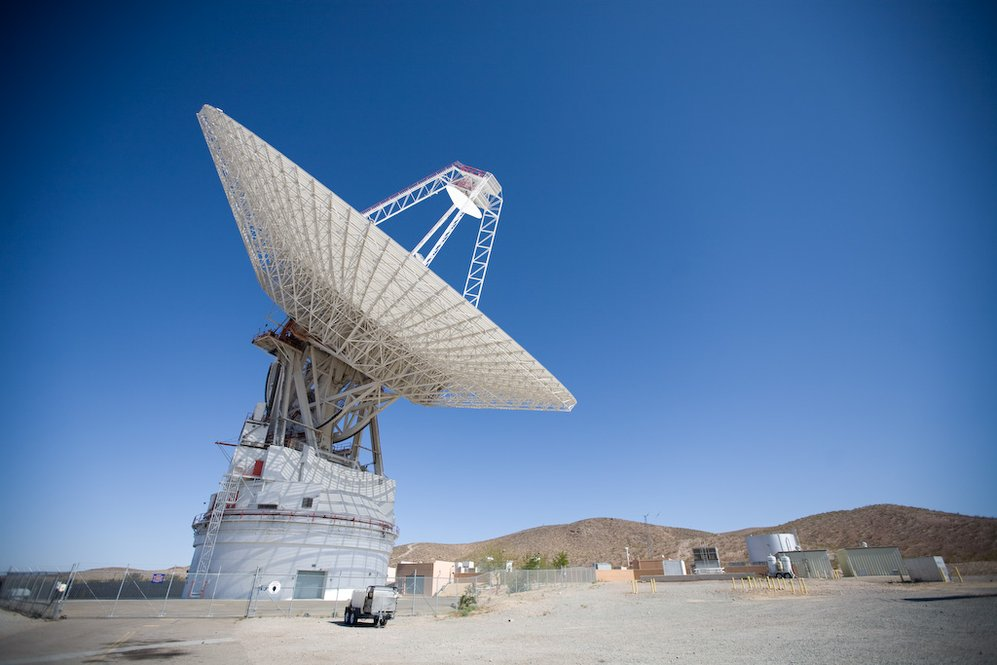
\includegraphics[scale=.3]{Goldstone.jpg}
\caption{Antenne der NASA Deep Space Network Einrichtung in Goldstone,
Kalifornien, USA}
\label{fig:Goldstone}
\end{figure}

\textbf{Interplanitary Internet}

Das IPN bezeichnet die Erweiterung des Internets auf einen au{\ss}erirdischen
Bereich. Die damit verbundenen {\"A}nderungen im Vergleich zum Irdischen
Internet umfassern z.B. einen gesonderten Umgang mit Latenzen, da diese beim IPN
im Minuten bis Stunden Bereich liegen. Die Entwicklung von Protokollen
f{\"u}r das IPN obliegt dabei dem Consultative Committee for Space Data Systems
(CCSDS).

\textbf{Delay Tolerant Networking}

DTN bezeichnet eine Protokollarchitektur f{\"u}r End-to-end Netzwerkverbindungen
mit geringer stabilit{\"a}t. Die Basis der DTN Netzwerkarchitektur stellt das
von der NASA entwickelte IPN (Interplanitary Internet) dar. Ein wichtiger
Bestandteil dieser Netzwerke ist der Umgang mit gro{\ss}en Latenzen. zudem
m{\"u}ssen die an der Kommunikation beteiligten Knoten (Teilnehmer) Daten so
lange zwischen bis der Empf{\"a}nger den erhalt quittiert hat
(store-and-forward).

\textbf{Bundle Protokolle}

Die in den RFCs 4838 und 5050 festgelegten Anforderungen f{\"u}r DTN sind
weitgehend unter der bezeichnung Bundle-Protokoll bekannt. In diesem werden Folgen von
Datenbl{\"o}cken als B{\"u}ndel zusammengefasst. Jedes B{\"u}ndel enth{\"a}lt
dabei ausreichende semantische Informationen um eine etwaige Applikation
fortzusetzen. Exemplarisch sei hier ein Webbrowser angef{\"u}hrt, welcher ein
Bundle-Paket erh{\"a}lt und dadurch eine Komplette Webseite anzeigt. Auch hier
erfolgt die {\"U}bertragung per store-and-forward. Die eingesetzten
Transportprotokolle k{\"o}nnen dabei variieren (IP basierend o.a.). Das
Bundle-Protokoll z{\"a}hlt zu den Overlay-Netzwerken, welche auf einer bereits
bestehenden Netzwerkstruktur aufsetzen.










